\chapter{Memorias}
\label{cap:memorias}

La memoria es un acto en el presente. En tal acto, tanto la imaginación como las experiencias, las competencias, las necesidades, los intereses, las emociones, los sentimientos y los sesgos personales no pueden no influir. Las expectativas personales y sociales también pesan en el presente acto de recordar. \emph{Recordar} es volver a pasar por el corazón, \emph{recordar} es volver a sonar. Con esto en mente, con la conciencia de que recordar es un acto creativo, intento traer a mi memoria tanto la primer reunión con las autoridades universitarias como la reunión entre «Pajarito», Juan Martín y yo.


\section{El canto y las palabras de un hijo}
\label{sec:palabra-canto}

\begin{figure}[H]
\centering
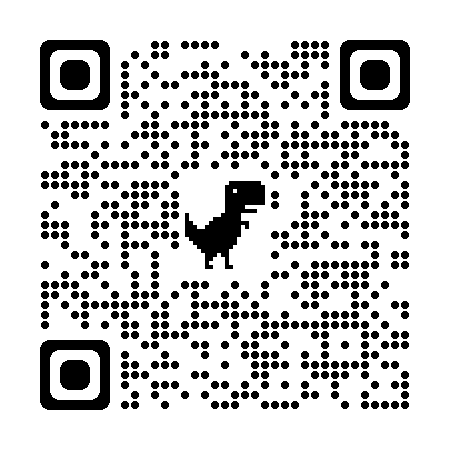
\includegraphics[width=0.3\textwidth]{img/qrcode-himno-memoria}
\caption{El canto y las palabras de \textsc{Juan Martín Leguizamón}.}
\label{fig:canto-palabras}
\end{figure}


En diciembre de 2022 me contacta \textsc{Marcelo «Pajarito» Sutti}\footnote{\textsc{Marcelo Sutti} es destacado poeta y músico salteño.}, quien me informa que \textsc{Juan Martín Leguizamón}\footnote{\textsc{Juan Martín Leguizamón}, hijo de Gustavo, es antropólogo y presidente de la Fundación Legado Cultural Cuchi Leguizamón.} le refiere tener viva en su memoria una melodía que recuerda bajo el título de \emph{Himno a la UNSa}. Enteradas las autoridades de la Universidad del relato de Juan Martín ---y mediado por Sutti quien me señala ante ellas como un hombre idóneo para realizar un peritaje sobre la melodía en memoria del hijo del «Cuchi»---, organizan una reunión en la que acordamos trabajar sobre el fragmento recordado y su posible relación con los modos de componer del legendario músico saleño. La posibilidad de establecer un grado de compatibilidad entre la melodía a estudiar y las melodías de Gustavo Leguizamón existe porque existen técnicas de análisis que pueden develar estructuras análogas en diversas piezas de un mismo autor. El \emph{análisis schenkeriano} en el particular caso me pareció una herramienta adecuada por ser capaz de mostrar estructuras intermedias y de superficie propias de un autor es específico, y es la que propuse en esa reunión utilizar en la pericia.

No recuerdo si primero fue la reunión con las autoridades universitarias, o si antes fue la reunión con Sutti y Leguizamón (h). No importa\footnote{La reunión con Sutti y Leguizamón (h) fue el 20 de diciembre de 2022 en mi domicilio particular y la grabación fue registrada a las 16:46 horas; con las autoridades nos reunimos el día 27 del mismo mes a las 16:00 horas en un bar del centro de la ciudad de Salta.}. Sí importa que fue una tarde de verano con un cielo tapado de amenazantes y negras nubes. El momento central de esa amena y nada amenazante charla no es necesario recordarlo: el registro electrónico nos exime del acto creativo de recordar, y él es accesible con el código QR de la Figura~\ref{fig:canto-palabras}.

\begin{figure}[htb]
\begin{ly}
\relative {
  \clef "treble"
  \key es \major
  \time 12/8
  \tempo 4.= 55
  \partial 8
  bes8
  es4. ~ es4 es8 es4 c8 ~ c d es
  f4. ~ f8 f es d4. r4 bes8
  g'4. ~ g4 g8 g4 es8 ~ es f g
  aes4. aes8 aes g f4. r4 bes8
  es4. ~ es4 es8 es4 c8 ~ c d es
  d4. ~ d8 bes g bes4. r
  c8 aes4 ~ aes aes8 aes f4 ~ f8 g aes
  g4. ~ g4 g8 g4 es8 ~ es f g
  f4. ~ f8 g f c4 d bes
  es2.
}
\end{ly}
\caption[Transcripción de un fragmento de la melodía recordada.]{Transcripción de la melodía recordada y cantada por \textsc{Juan Martín Leguizamón.}}
\label{fig:Transcripcion}
\end{figure}

Basta con transcribir un fragmento de lo cantado por el hijo del «Cuchi» para detectar una serie de significativas características, algunas que acercan esta versión a la versión escrita (mostrada y estudiada en el Capítulo~\ref{cap:partitura}), otras que producen la divergencia entre ellas.

La tonalidad de Mi\bemoltxt mayor utilizada por Juan Martín ---a diferencia de la de Fa mayor consignada en la partitura--- es debido a que para su registro de voz ---y no sólo para el de él, sino para el registro vocal de la mayoría de la población--- esta tonalidad es más conveniente. La melodía escrita por su padre, en Fa mayor, es de difícil canto para la mayoría de la etnia de Salta. Sin embargo, en amplio pasaje las dos versiones coinciden en su conformación interválica, reconociéndose en la versión de Juan Martín la pieza de Gustavo Leguizamón. A tal punto es así que el 23 de abril de 2023 a la tarde, consultado yo telefónicamente por \textsc{Lucrecia Coscio}\footnote{Coordinadora del Centro Cultural Holver Martínez Borelli de la UNSa.} acerca de si algunas de las partituras que me enviaba vía \emph{WhatsApp} tenía relación con la melodía referida por Juan Martín.

\begin{figure}[htb]
\centering
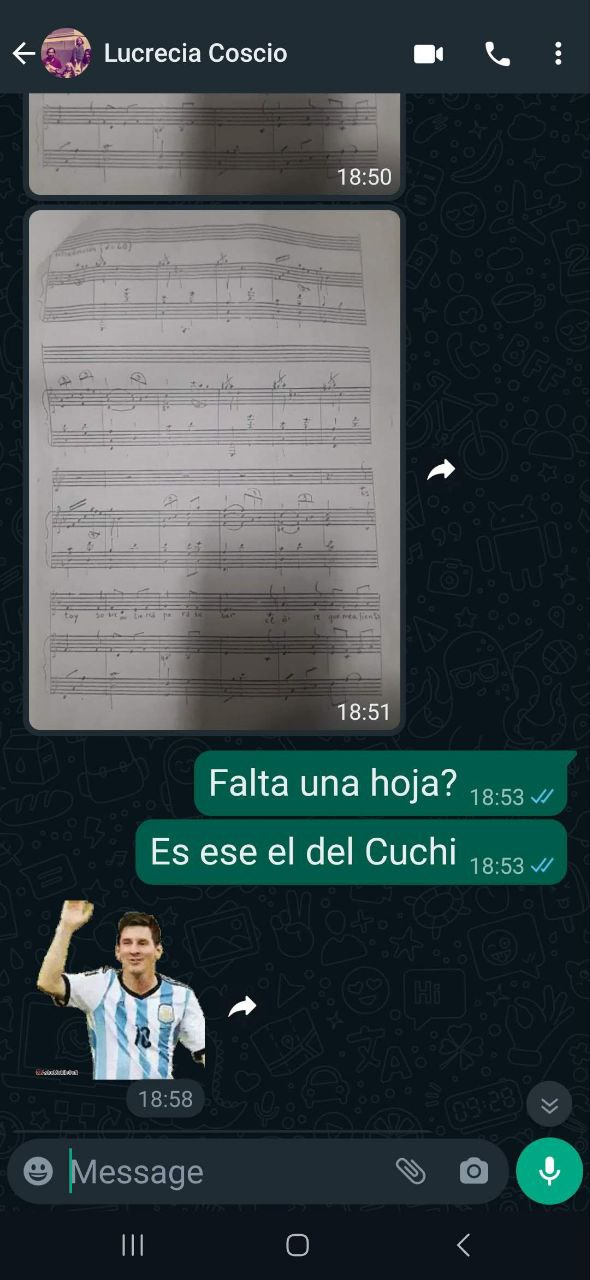
\includegraphics[width=0.4\textwidth]{img/lucrecia1}
\caption{21 de abril: hallazgo de la partitura.}
\label{fig:hallazgo-partitura}
\end{figure}

\noindent Ese mismo día, en horas de la mañana, la profesora Coscio me había enviado otras partituras que indudablemente no tenían relación con la melodía en cuestión, y así lo hice saber. Pero faltando 12 minutos para las 19:00 horas, Lucrecia vuelve a comunicarse conmigo. Mientras me dirijo a la presentación de la flamante \emph{Fundación Legado Cultural Cuchi Leguizamón} veo las fotos y reconozco de inmediato el parentesco de lo que está escrito con lo cantado durante una tormenta de verano cuatro meses atrás: es el himno del «Cuchi»\footnote{Esa misma tarde, junto a la partitura se halló un sobre conteniendo los datos de los autores de la letra y la música (ver Figura~\ref{fig:sobre-letra} en la página~\pageref{fig:sobre-letra}).}. Gol.


\section{La memoria oral y la memoria escrita}
\label{sec:memoria-oral-escrita}



% TODO
%
% diferencias sustanciales
%
% rigidez compu en 2/4, mas no en 12/8. ¿Cómo será, no?
